\section{Methods}

\subsection{Parsing LTL formulae}
% Include abstract syntax tree
% Make the grammar unambiguous here
Parsing an LTL formula from a text based representation into an abstract syntax tree (AST) is performed using a top-down parser with the recursive decent algorithm. The recursive descent algorithm follows the structure of the context-free grammar closely by having a mutually exclusive procedure for each non-terminal production rule in the grammar. Care has to be taken to uphold the left- and right-associative rules for each of the operators. In \autoref{alg:recursive-descent} the overall structure of the recursive descent algorithm can be seen for the $i$'th production rule.
\begin{algorithm}[H]
\SetAlgoLined
\DontPrintSemicolon
\SetKwProg{rd}{Algorithm}{}{}
\rd{$rd_i()$}{
    $lhs := rd_{i+1}()$\;
    \If{$token \in scanner$}{
        \KwRet $op\{lhs, rd_i()\}$
    }
    \KwRet lhs
}{}

\caption{The recursive descent algorithm for the $i$'th production rule}
\label{alg:recursive-descent}
\end{algorithm}
A procedure for the $i'th$ production rule generally parses its left-hand side with the production rule following itself (i.e. the production rules with higher associativity). The procedure then recurses on the right hand side, as long as the operator matching the current production rule can be found in the input stream. Recursing on the right-hand side makes the parsing right-associative. 

\begin{example}
We consider the AST for the formula $\phi = a \U b \land c$ which can be seen in \autoref{fig:ast-exampl1}. The precedence rule of the until operator ($\U$) is stronger than that of the logical and operator ($\land$), which is explicitly shown in the AST.
\begin{figure}[!ht]
    \centering
    \begin{forest}
for tree={draw, minimum size=5mm, anchor=center}  
[$\land$,
    [$\U$,
        [$a$]
        [$b$]
    ]
    [$c$]
]
\end{forest}
    \caption{The AST for $\phi = a \U b \land c$}
    \label{fig:ast-exampl1}
\end{figure}
\end{example}

\begin{example}
We consider the AST for the formula $\phi = a \U b \U c$ which can be seen in \autoref{fig:ast-exampl2}. Because the until operator ($\U$) is right-associative, which is conveyed by the AST, the subformula $b \U c$ is evaluated first, and therefore not the root of the tree.

\begin{figure}[!ht]
    \centering
    \begin{forest}
        for tree={draw, minimum size=5mm, anchor=center}  
        [$\U$,
            [$a$]
            [$\U$,
                [$b$]
                [$c$]
            ]
        ]
    \end{forest}
    \caption{The AST for $\phi = a \U b \U c$}
    \label{fig:ast-exampl2}
\end{figure}
\end{example}

\subsection{Checking for Satisfiability}

\subsubsection{Determining Elementary Sets}
\label{sec:method-elemesets}
The problem of finding elementary sets is essential in model checking of LTL formulae. In this paper are two methods presented for determining the elementary sets of an LTL formula, the first being a naive approach and the second being an optimised decision tree based approach.

\paragraph{Naive approach}
% Describe approach
In the naive approach for finding elementary sets all subsets of the closure of $\phi$ is considered to be elementary or not. Since all subsets of $closure(\phi)$ are considered, the naive approach does not exclude any sets which are trivially not elementary, i.e. sets which are not maximal. Since $|closure(\phi)|$ is $\mathcal{O}(|\phi|)$ the number of possible elementary sets which is considered by the naive approach is $\mathcal{O}(2^{|\phi|})$. Checking whether a set is elementary or not takes $\mathcal{O}(|\phi|)$ time which results in a total time complexity of $\mathcal{O}(2^{|\phi|} \cdot |\phi|)$.

\paragraph{Decision tree approach}
% Describe approach
The decision tree based approach exploits the property of elementary sets being maximal, i.e. for all $\psi \in closure(\phi)$:
\begin{equation*}
  \psi \notin B \imply \lnot \psi \in B \tag{\autoref{eq:elem3.1}}
\end{equation*}
This very fundamental property leads to a binary relationship for each subformula, where either the negated or the non-negated subformula must be present in the elementary set. The algorithm considers all subformulae $\psi$ of $\phi$ in ascending order of their formula length $|\phi|$. This results in the smallest subformulae being considered prior to any other subformula. The algorithm proceeds as follows: 

Let $\mathcal{S}$ be the list of subformulae $\psi$ of $\phi$ sorted in ascending order according to $|\psi|$. The algorithm recursively explores a decision tree $\mathcal{T}$ where a node at depth $i$ will have one edge exploring the $i$'th element of $\mathcal{S}$ and another edge exploring the negation of the $i$'th element of $\mathcal{S}$. A node is marked inconsistent if the path $\pi$ from the root node to the node itself (corresponding to a set of subformulae) is inconsistent with respect to propositional logic (\autoref{eq:elem1.1} - \autoref{eq:elem1.3}) or inconsistent with respect to the until operator (\autoref{eq:elem2.1} and \autoref{eq:elem2.2}). An inconsistent node halts further exploration, as an inconsistent node can not reach a state where it becomes consistent again. The decision tree $\mathcal{T}$ is complete when all subformulae of $\mathcal{S}$ has been considered. The elementary sets are then the root to leaf paths $\pi$ of which there are no inconsistent nodes.

Since the height of the decision tree is $\mathcal{O}(|\phi|)$ and the tree is binary, the time complexity for exploring the decision tree is $\mathcal{O}(2^{|\phi|})$. Although the time complexity is still exponential with respect to $|\phi|$ like the naive approach, the algorithm shows vast improvements in practice because of the early elimination of inconsistent nodes.

Now remains the problem of determining if a path $\pi$ from the root to any node $\mathcal{N}$ is inconsistent. The property of consistency is upheld by satisfying the properties in \autoref{sec:elemesets}, namely the rules for logical consistency (\autoref{eq:elem1.1} - \autoref{eq:elem1.3}) and the rules for local consistency (\autoref{eq:elem2.1} and \autoref{eq:elem2.2}). The property of maximality (\autoref{eq:elem3.1}) is already inherently upheld by the structure of the decision tree. We now show that consistency is upheld by the following proof:

\begin{proof}
We start of by proving that for any path $\pi=\pi_0,\ldots,\pi_n$ in the decision tree, the set consisting of the subformulae on the path $\pi$ is elemental with respect to the closure $closure(\pi)$. By $closure(\pi)$ we mean all subformulae on the path $\pi$ and their negations. Specifically we want to show that \autoref{eq:elem1.1}, \autoref{eq:elem1.3}, \autoref{eq:elem2.1} and \autoref{eq:elem2.2} holds. These properties are upheld by the ordering of $\mathcal{S}$ and the definition of consistency for elementary sets (\autoref{sec:elemesets}). The remaining properties, \autoref{eq:elem1.2} and \autoref{eq:elem3.1}, is later proven by the structure of the decision tree.

We start by considering \autoref{eq:elem1.1}. Assume that this property does not hold for $closure(\pi)$. Then we must have one of two scenarios:
\begin{itemize}
    \item $\phi_1 \land \phi_2 \in B \land \lnot(\pi_1 \in B \text{ and } \phi_2 \in B)$ \quad
    Because of the ordering of $\mathcal{S}$ and that $|\phi_1 \land \phi_2| < |\phi_1|$ and $|\phi_1 \land \phi_2| < |\phi_2|$, we know that $\phi_1$ and $\phi_2$ must be on the path $\pi$ before $\phi_1 \land \phi_2$. Otherwise the path would have been marked inconsistent, and the path would not exist. This contradicts the assumption.
    \item $\phi_1 \land \phi_2 \notin B \land \pi_1 \in B \text{ and } \phi_2 \in B$ \quad This case is trivially a contradiction, because such a path would have been marked inconsistent.
\end{itemize}
\autoref{eq:elem1.3} is trivial and can be proven in a similar manner. We now proceed to consider \autoref{eq:elem2.1}. Assume that this property does not hold for $closure(\pi)$. Then we must have the following scenario:
\begin{itemize}
    \item $\phi_2 \in B \land \phi_1 \U \phi_2 \notin B$ \quad
    Again we exploit the ordering of $\mathcal{S}$. We therefore know $\phi_2$ to be on the path prior to $\phi_1 \U \phi_2$. Then this path would not exist since it would have been marked as inconsistent. This contradicts our assumption.
\end{itemize}
Lastly we consider \autoref{eq:elem2.2}. Assume that this property does not hold for $closure(\pi)$. Then we have the following scenario:
\begin{itemize}
    \item $\phi_1 \U \phi_2 \in B \land \phi_2 \notin B \land \pi_1 \notin B$ \quad Again because of the ordering of $\mathcal{S}$ $\phi_1$ and $\phi_2$ must appear on the path before $\phi_1 \U \phi_2$. Then this path would have been marked inconsistent and not exist.
\end{itemize}

It now remains to show that \autoref{eq:elem1.2} and \autoref{eq:elem3.1} holds under the structure of the decision tree. Consider a path $\pi$ in the completely explored decision tree from the root node to a leaf node. We set out to prove that $\pi$ corresponds to a maximal set of subformulae which satisfies \autoref{eq:elem1.2}. We prove this by contradiction. Assume that \autoref{eq:elem1.2} does not hold for some path $\pi$, meaning:
\begin{equation*}
    \psi \in B \land \lnot \psi \in B \tag{contradiction of \ref{eq:elem1.2}}
\end{equation*}
Then $\psi$ must belong to some edge $\pi_i$ in $\pi = \pi_0, \ldots, \pi_{i-1}, \pi_i, \pi_{i+1},\ldots,\pi_n$. Since each subformula of $\mathcal{S}$ is considered exactly once, $\psi$ and $\lnot \psi$ must correspond to the same element of $\mathcal{S}$. The subtree containing $\psi$ must therefore be disjoint from the subtree containing $\lnot\psi$, thus no path can contain both. This contradicts our assumption.
For the case of maximality we again consider the following contradiction. Assume that the rule of maximality, \autoref{eq:elem3.1}, does not hold, meaning:
\begin{equation*}
    \psi \notin B \land \lnot \psi \notin B \tag{contradiction of \ref{eq:elem3.1}}
\end{equation*}
Then $\psi$ must not be on the path $\pi$. We however know that $\pi$ has a length of $|\mathcal{S}|$ (else it would have been marked inconsistent) and thus must pass through exactly one edge at each depth of the tree. Since $\psi$ must belong to $\mathcal{S}$ and a node at depth $i$ considers the $i$'th element of $\mathcal{S}$, then $\pi$ must contain either $\psi$ or $\lnot\psi$. this contradicts our assumption.

Because we have shown the elementary set properties to hold for a path $\pi$ with respect to $closure(\pi)$ we lastly note that any path $\pi$ of length $|\mathcal{S}|$ is an elementary set with respect to $closure(\pi)=closure(\phi)$.
\end{proof}

\begin{example}
We now consider the decision tree algorithm for finding elementary sets for $\phi = a \cup (a \land b)$. In figure~\ref{fig:elemset} the fully explored decision tree can be seen. Nodes which have been marked as inconsistent are displayed as a cross.
\begin{figure}[!ht]
\begin{center}
    \begin{forest}
for tree={circle, draw, s sep=14pt}
[, 
    [,edge label={node[midway,left] {$a$}}  
      [,edge label={node[midway,left] {$b$}}
        [,edge label={node[midway,left] {$a \land b$}}
            [,edge label={node[midway,left] {$\varphi$}}]
            [,cross out, edge label={node[midway,right] {$\lnot\varphi$}}]
        ]
        [,cross out, edge label={node[midway,right] {$\lnot (a \land b)$}}
            [,draw=none,edge={draw=none}]
            [,draw=none,edge={draw=none}]
        ] 
      ] 
      [,edge label={node[midway,right] {$\lnot b$}}
        [,cross out, edge label={node[midway,left] {$a \land b$}}
            [,draw=none,edge={draw=none}]
            [,draw=none,edge={draw=none}]
        ] 
        [, edge label={node[midway,right] {$\lnot (a \land b)$}}
            [,edge label={node[midway,left] {$\varphi$}}]
            [,edge label={node[midway,right] {$\lnot\varphi$}}]
        ] 
      ] 
    ]
    [,edge label={node[midway,right] {$\lnot a$}}
      [,edge label={node[midway,left] {$b$}}
        [,cross out, edge label={node[midway,left] {$a \land b$}}
            [,draw=none,edge={draw=none}]
            [,draw=none,edge={draw=none}]
        ]
        [,edge label={node[midway,right] {$\lnot (a \land b)$}}
            [,cross out, edge label={node[midway,left] {$\varphi$}}]
            [,edge label={node[midway,right] {$\lnot\varphi$}}]
        ] 
      ] 
      [,edge label={node[midway,right] {$\lnot b$}}
        [,cross out, edge label={node[midway,left] {$a \land b$}}
            [,draw=none,edge={draw=none}]
            [,draw=none,edge={draw=none}]
        ]
        [,edge label={node[midway,right] {$\lnot (a \land b)$}}
            [,cross out, edge label={node[midway,left] {$\varphi$}}]
            [,edge label={node[midway,right] {$\lnot\varphi$}}]
        ]
      ]  
  ] 
]
\end{forest}
    \caption{Decision tree for formula $a \U (a \land b)$}
    \label{fig:elemset}
\end{center}
\end{figure}
After exploration of the decision tree one can find the elementary sets of $\phi$ as the root to leaf paths not containing any inconsistent nodes. This results in the following elementary sets:
\begin{align*}
    B_1 &= \{a,         b,         a\land b,           \phi\} \\
    B_2 &= \{a,         \lnot b,    \lnot (a\land b),   \phi\} \\
    B_2 &= \{a,         \lnot b,    \lnot (a\land b),   \lnot \phi\} \\
    B_4 &= \{\lnot a,   b,         \lnot (a\land b),  \lnot \phi\} \\
    B_5 &= \{\lnot a,   \lnot b,    \lnot (a\land b),   \lnot \phi\} \\
\end{align*}
\end{example}

\subsubsection{GNBA}
The method of model checking the confidentiality and integrity policies involves constructing a generalised non-deterministic Büchi automaton (GNBA) over the formula $\lnot\phi$ (read; the negation of phi). The GNBA functions as a monitor for the transition system for which its accepting states serves to disprove the formula $\phi$. If the formula can not be disproved, hence no counterexample of $\phi$ can be found, it is said to be valid. The states of the GNBA is comprised of the elementary sets of $\phi$ of which we have discussed in \autoref{sec:method-elemesets}. The GNBA has at most $2^{|\phi|}$ states where the number of acceptance state sets equals the number of until formulae in $\phi$. We say that for a LTL formula $\phi$ there exists a GNBA $\mathcal{G_\phi}$ where $Words(\phi)=\mathcal{L}_\omega(\mathcal{G_\phi})$. The construction of the GNBA is formalised as follows:
\begin{definition}[Construction of GNBA from LTL\cite{baier2008principles}]
\label{def:ltl-to-gnba}
Given an LTL formula $\phi$ over AP a GNBA $\mathcal{G}=(Q,2^{AP},\delta,Q_0,\mathcal{F})$ can be constructed in space and time $\mathcal{O}(2^{|\phi|})$ as follows:
\begin{itemize}
    \item $Q = B \subseteq closure(\phi) \mid \text{ set is elementary}$,
    \item $Q_0 = \{ B \in Q \mid \phi \in B \}$,
    \item $\mathcal{F} = \{F_{\phi_1 \U \phi_2} \mid \phi_1 \U \phi_2 \in closure(\phi)\} \text{ where }$
    \begin{equation*}
        F_{\phi_1 \U \phi_2} = \{B \in Q \mid \phi_1 \U \phi_2 \not\in B \text{ or } \phi_2 \in B\}
    \end{equation*}
\end{itemize}
With the transition function $\delta : Q \times 2^{AP} \imply 2^Q$:
\begin{itemize}
    \item If $A \neq B \cap AP$, then $\delta(B,A)=\varnothing$
    \item If $A = B \cap AP$, then $\delta(B,A)$ is the set of every $B'\in Q$ satisfying
    \begin{enumerate}
        \item for every $\X\psi \in closure(\phi)$: $\X\psi \in B \biimply \psi \in B'$, and
        \item for every $\psi_1 \U \phi_2 \in closure(\phi)$:
        \begin{equation*}
            \phi_1 \U \phi_2 \in B \quad\biimply\quad (\phi_2 \in B \lor (\phi_1 \in B \land \phi_1 \U \phi_2 \in B'))
        \end{equation*}
    \end{enumerate}
\end{itemize}
\end{definition}

\begin{example}
We consider the confidentiality policy from Example~\ref{ex:mutual-exclusion} with the formula $\conf = \G(\lnot a \lor \lnot b)$ and the construction of the GNBA $\mathcal{G}_\phi$. First the formula is negated and then transformed.
\begin{equation*}
    \phi = \lnot \conf = \lnot \G(\lnot a \lor \lnot b) \quad\Longleftrightarrow\quad true \U (a \land b)
\end{equation*}
We then determine the elementary sets of $\phi$:
\begin{align*}
    B_1 &= \{\lnot a, b, true, \lnot(a \land b), \lnot\phi\} \\
    B_2 &= \{a, \lnot b, true, \lnot(a \land b), \lnot\phi\} \\
    B_3 &= \{\lnot a, \lnot b, true, \lnot(a \land b), \lnot\phi\} \\
    B_4 &= \{a, b, true, a \land b, \phi\} \\
    B_5 &= \{\lnot a, b, true, \lnot(a \land b), \phi\} \\
    B_6 &= \{a, \lnot b, true, \lnot(a \land b), \phi\} \\
    B_7 &= \{\lnot a, \lnot b, true, \lnot(a \land b), \phi\}
\end{align*}
The GNBA can now be constructed following \autoref{def:ltl-to-gnba} which can be seen in \autoref{fig:gnba-example1}. Lets inspect the state $B_4$ in more detail. The set of atomic propositions with which one can move from this state is $B_4 \cup AP = \{a,b\}$. Since $true \U (a \land b) \in B_4$ and $a \land b \in B_4$, the transition function trivially returns $Q$, thus $B_4$ can transition to all states.

\begin{figure}[!ht]
    \centering
    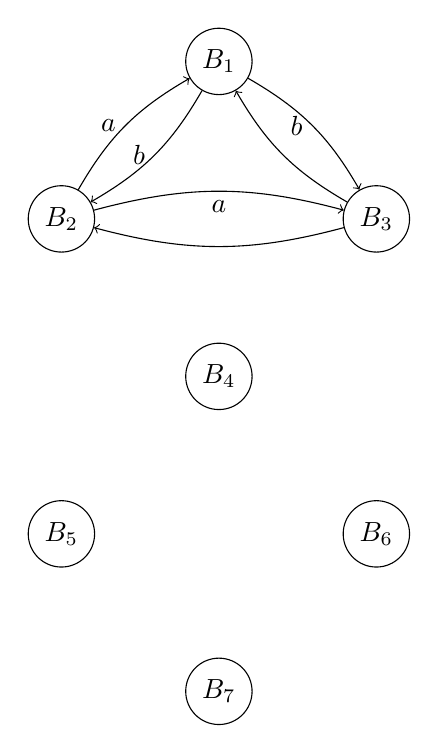
\begin{tikzpicture}
    \node[shape=circle,draw=black] (B1) at (0,0) {$B_1$};
    \node[shape=circle,draw=black] (B2) at (-2,-2) {$B_2$};
    \node[shape=circle,draw=black] (B3) at (2,-2) {$B_3$};
    \node[shape=circle,draw=black] (B4) at (0,-4) {$B_4$};
    \node[shape=circle,draw=black] (B5) at (-2,-6) {$B_5$};
    \node[shape=circle,draw=black] (B6) at (2,-6) {$B_6$};
    \node[shape=circle,draw=black] (B7) at (0,-8) {$B_7$};

    \path [->] (B1) edge[bend left=15] node[left] {$b$} (B2);
    \path [->] (B2) edge[bend left=15] node[left] {$a$} (B1);
    
    \path [->] (B1) edge[bend left=15] node[left] {$b$} (B3);
    \path [->] (B3) edge[bend left=15] node[left] {$\varnothing$} (B1);
    
    \path [->] (B3) edge[bend left=15] node[above] {$\varnothing$} (B2);
    \path [->] (B2) edge[bend left=15] node[below] {$a$} (B3);

\end{tikzpicture}
    \caption{The GNBA for $\phi=true\U (a \land b)$}
    \label{fig:gnba-example1}
\end{figure}
\end{example}

\subsubsection{NBA}
The non-deterministic Büchi automaton (NBA) is derived from the GNBA by a well-defined transformation. The equivalent NBA accepts the same language as the GNBA but simplifies the model checking algorithm. We say that for a GNBA $\mathcal{G}$ there exists a NBA $\mathcal{A}$ such that $\mathcal{L}_\omega(\mathcal{G})=\mathcal{L}_\omega(\mathcal{A})$. The transformation for $\mathcal{G}=(Q,\Sigma,\delta,Q_0,\mathcal{F})$ and $\mathcal{F}=\{F_1,\ldots,F_k\}$ is constructed by creating $k$ copies of the GNBA. Then, for the $i$th copy, the acceptance states are connected to the equivalent states in the $(i+1)$th copy. Because a run can only move from the $i$th copy to the next through an acceptance state $q \in F_i$, the construction ensures that an accepting run visits an acceptance state in each copy infinitely often. The construction of the NBA $\mathcal{A}=(Q',\Sigma',\delta',Q_0',F')$ is formalised as follows:

\begin{definition}[Construction of NBA from GNBA]
Given an GNBA an equivalent NBA can be constructed in time and space $\mathcal{O}(|\mathcal{G}|\cdot|\mathcal{F}|)$. Let $\mathcal{G}=(Q,\Sigma,\delta,Q_0,\mathcal{F})$ with acceptance states $\mathcal{F}=\{F_1,\ldots,F_k\}$ then the NBA $\mathcal{A}=(Q',\Sigma',\delta',Q_0',F')$ can be constructed as:
\begin{itemize}
    \item $Q'=Q\times \{1,\ldots,k\}$,
    \item $Q_0'=Q_0 \times \{1\} = \{\langle q_0,1 \rangle \mid q_0 \in Q_0\}$, and
    \item $F'=F_1 \times \{1\} = \{\langle q_F,1 \rangle \mid q_F \in F_1\}$
\end{itemize}
With the transition relation:
\begin{equation*}
    \delta'(\langle q,i \rangle, A)=
    \begin{cases*}
      \{\langle q',i \rangle \mid q' \in \delta(q,A)\} & if $q \not\in F_i$ \\
      \{\langle q',i+1 \rangle \mid q' \in \delta(q,A)\}        & otherwise
    \end{cases*}
\end{equation*}
\end{definition}

\subsubsection{Product Automaton}
\label{sec:product-automaton}
The product automaton $TS \otimes A$ is constructed from the transition system $TS$ and the automaton $A$ over $\phi$ by constructing every possible pair of states from both systems with some relation function between states. This results in at most $|TS|\cdot |A|$ states. The intuitive understanding of the product is to combine all paths in $TS$ with all runs of $A$. The problem of checking $\phi$ is the reduced to checking whether $Traces(TS) \cap \mathcal{L_\omega}(A) \neq \varnothing$. We prove this by finding a path in the product for which an accepting state of $A$ is visited infinitely often. This path is then a counter example for $TS \not\models \phi$. If no counter example is found, then $\phi$ is proved to hold.

\subsubsection{Nested Depth-First Search}
% Maintain a set next to the stack for constant time lookup
The problem of determining $Traces(TS) \cap \mathcal{L_\omega}(A) \neq \varnothing$, as described above, \autoref{sec:product-automaton}, results in checking whether a path exists in $TS \otimes A$ which visits an acceptance state infinitely often. Finding such a path is achieved with a nested depth-first search (NDFS). The algorithm is structured in an outer and inner depth-first search (DFS) for which the outer DFS searches to find an accepting state and the inner DFS searches to find a cycle. If such a cycle can be found one can conclude that the accepting state can be visited infinitely often, proving $TS \not\models \phi$. If the outer DFS manages to explore all accepting states with no accepting cycles in the inner DFS, then no counter example can be found, thus $TS \models \phi$ is proved.
\begin{algorithm}[H]
\SetAlgoLined
\DontPrintSemicolon
\SetKwProg{dfs}{Algorithm}{}{}
\dfs{dfs(s)}{
    $P = S \cup \{s, 0\}$\;
    $\textit{push}(S,s)$\;
    \For{$t \in successors(s)$}{
        \If{$\{t,0\} \not\in P$}{
            $\textit{dfs}(t)$
        }
        \If{$s \in acceptance$}{
            $\textit{ndfs}(s)$
        }
        $pop(T)$\;
    }
}{}\;

\SetKwProg{ndfs}{Procedure}{}{}
\ndfs{ndfs(s)}{
    $P = P \cup \{s, 1\}$\;
    $\textit{push}(T,s)$\;
    \For{$t \in successors(s)$}{
        \uIf{$t \in S$}{
            \KwRet true\;
        }\uElseIf{$\{t,1\} \not\in P$}{
            $\textit{ndfs}(t)$
        }
    }
    $\textit{pop}(T)$
}{}
\caption{Cycle detection algorithm using nested DFS}
\label{alg:ndfs}
\end{algorithm}
In \autoref{alg:ndfs} the algorithm for NDFS can be seen. The algorithm is structured as two recursive DFS algorithms, one for the outer and one for the inner DFS. The outer DFS will search recursively until no more successors can be recursed, then call the NDFS procedure on all acceptance states as the recursion unfolds. By postponing the inner DFS one can limit the number of states recursed by the inner DFS before finding a cycle, as the inner recursion searches until it hits the stack from the outer DFS, in which case a cycle has been found. 

